\documentclass{article}

\usepackage{tikz}

\usetikzlibrary[arrows.meta,calc,positioning]

\title{Admin, Friend, Referred PKI v0.2}
\author{Wade T. Cline}

\begin{document}
\begin{abstract}
The ``Admin, Friend, Referred'' (AFR) Public Key Infrastructure (PKI) allows two-way authentication and authorization between servers and clients.  Clients can consist of either the admin, ``friends'' whom the admin invites, and ``referreds'' whom the admin's friends invite.  The \texttt{afr} tool has been developed in order to help the admin manage their part of AFR PKI and the \texttt{afrc} tool has been developed in order to help friends and referreds do the same.  The PKI is still in a prototype state and future work will involve solving the ``Admin revokes referred certificate'' use case, possibly with indirect Certificate Revocation Lists (CRLs).  A network protocol for managing the PKI will likely be critical for usability and thus adoption of the PKI.
\end{abstract}

\section{Introduction}
This paper will describe the ``Admin, Friend, Referred'' Public Key Infrastructure (PKI).  The PKI is designed in order to allow individual server admins to provide a secured service to a reasonably limited audience.  The below sections will elaborate on this purpose and then explain the solution adopted by the PKI.  Following sections will detail the structure of the X.509 certificates used for this solution and the terminology used to describe the various kinds of certificates used by the PKI.  Use Cases for the certificates are then defined and explained in terms of the certificate structure.  Tooling to assist in implementing the use cases is then documented.  The previous implementation of the certificate layout, called ``Friend-of-Friend'', and its shortcomings are then explained.  Finally, various items for future work are speculated upon based on their perceived usefulness.

\subsection{Problem Statement}
A perennial topic for discussion on the Internet is the creation of \emph{distributed} (or \emph{federated}) services.  Distributed services can provide a number of benefits, such as 1) autonomy, 2) censorship resistance, and 3) a robust infrastructure.  Unfortunately, actually implementing distributed services leads to a large number of problems.  Though all men may be created equal, their skills as system administrators are certainly not equal, and only a few posses the experience to competently provide a digital service.  Thus it falls to a few to provide for many.

Yet how many users should one provide for, and how will one supply the means to provide for them?  Large numbers of users require powerful equipment and constant moderation.  These things cost money, but users are often cheap and unwilling to pay for services.  One option is to monetize via advertising, but advertising tends to be alienating and privacy-invasive.  Another option is to provide the service free of charge, but a large number of demanding users tends to quickly exhaust an administrator's charity.  Likewise, the larger the userbase, the higher the likelihood for shady and unscrupulous individuals which will increase the moderation burden on the administrator; yet too small of a userbase means that no one is interested in using the service.  The administrator thus needs a way to manage their userbase in a reasonable manner.

\subsection{Proposed Solution}
In order to address the userbase issue, a solution of semi-controlled expansion using the X.509 client certificates provided as part of a Secure Sockets Layer (SSL) / Transport Layer Security (TLS) PKI is proposed.  There are three categories of user as part of the PKI: the \emph{admin}, who is the administrator of the server; a \emph{friend}, a user who is invited by the admin; and \emph{referred} users, who are invited by friends.  Allowing friends to refer users to the service allows for limited growth while ensuring that any new user must be vetted either by the admin or someone whom the admin knows.  Using X.509 certificates for authentication and authorization allows the proposed solution to work with any TCP/IP connection and to make use of already widely-deployed SSL/TLS libraries.  Thus the solution can limit growth to what is intended to be tolerable to an admin and can also be widely-deployed without the burden of additional software.

\section{Structure}
Figure \ref{fig:afr} illustrates the certificate layout used by the current version of AFR.
\begin{figure}
\begin{center}
\rotatebox{270}{
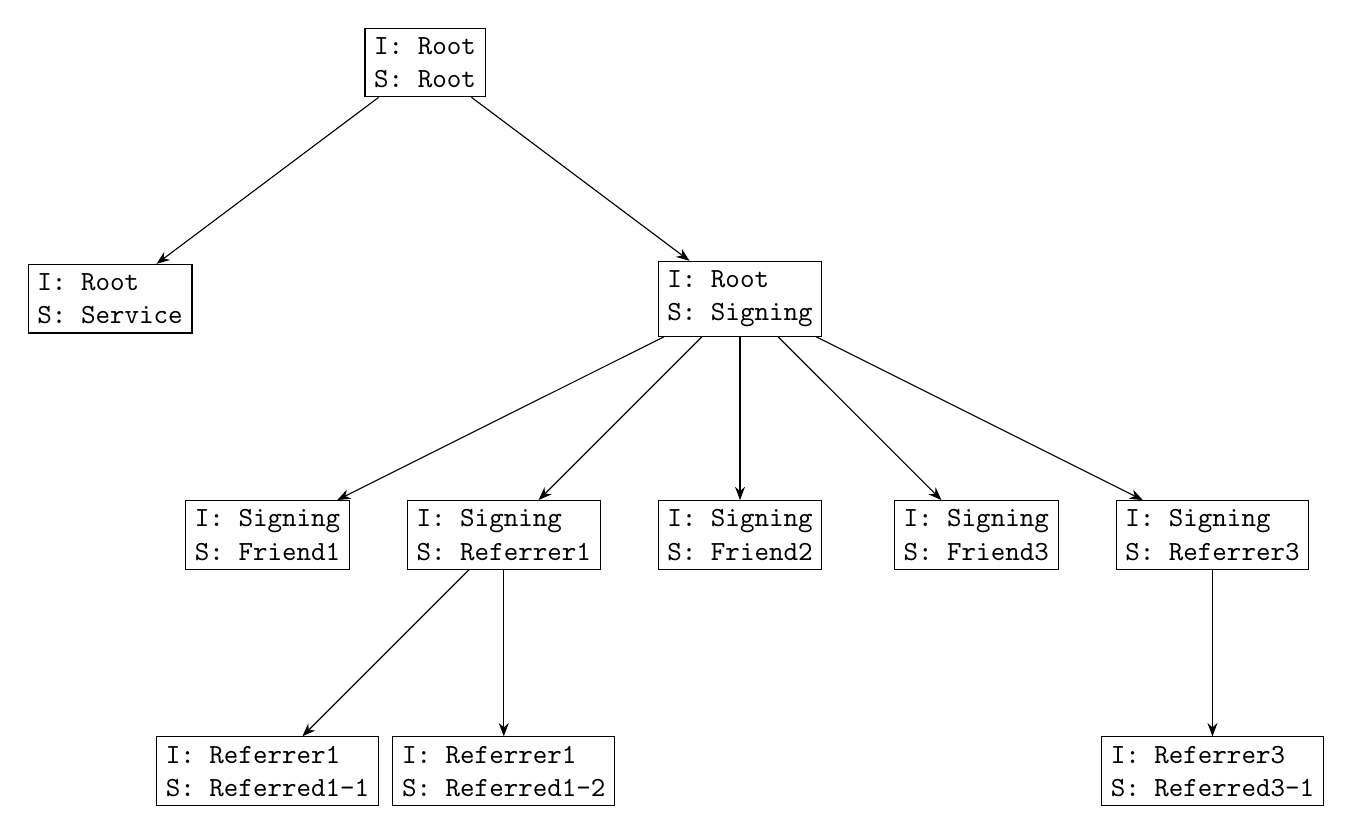
\begin{tikzpicture}
	\node (Root) at (0, 0) [align=left,draw] {\texttt{I: Root} \\ \texttt{S: Root}};

	\node (Service) at ($(Root) + (-4, -3)$) [align=left,draw] {\texttt{I: Root} \\ \texttt{S: Service}};
	\node (Signing) at ($(Root) + (4, -3)$) [align=left,draw] {\texttt{I: Root} \\ \texttt{S: Signing}};
	\draw[-Stealth] (Root) -- (Service);
	\draw[-Stealth] (Root) -- (Signing);

	\node (Friend1) at ($(Signing) + (-6, -3)$) [align=left,draw] {\texttt{I: Signing} \\ \texttt{S: Friend1}};
	\node (Referrer1) at ($(Signing) + (-3, -3)$) [align=left,draw] {\texttt{I: Signing} \\ \texttt{S: Referrer1}};
	\node (Friend2) at ($(Signing) + (0, -3)$) [align=left,draw] {\texttt{I: Signing} \\ \texttt{S: Friend2}};
	\node (Friend3) at ($(Signing) + (3, -3)$) [align=left,draw] {\texttt{I: Signing} \\ \texttt{S: Friend3}};
	\node (Referrer3) at ($(Signing) + (6, -3)$) [align=left,draw] {\texttt{I: Signing} \\ \texttt{S: Referrer3}};
	%\node (FriendExtra) at ($(Signing) + (9, -3)$) [align=left,draw] {\ldots};
	\draw[-Stealth] (Signing) -- (Friend1);
	\draw[-Stealth] (Signing) -- (Referrer1);
	\draw[-Stealth] (Signing) -- (Friend2);
	\draw[-Stealth] (Signing) -- (Friend3);
	\draw[-Stealth] (Signing) -- (Referrer3);
	%\draw[-Stealth] (Signing) -- (FriendExtra);

	\node (Referred1-1) at ($(Referrer1) + (-3, -3)$) [align=left,draw] {\texttt{I: Referrer1} \\ \texttt{S: Referred1-1}};
	\node (Referred1-2) at ($(Referrer1) + (0, -3)$) [align=left,draw] {\texttt{I: Referrer1} \\ \texttt{S: Referred1-2}};
	%\node (Referred1-Extra) at ($(Referrer1) + (3, -3)$) [align=left,draw] {\ldots};
	\node (Referred3-1) at ($(Referrer3) + (0, -3)$) [align=left,draw] {\texttt{I: Referrer3} \\ \texttt{S: Referred3-1}};
	\draw[-Stealth] (Referrer1) -- (Referred1-1);
	\draw[-Stealth] (Referrer1) -- (Referred1-2);
	%\draw[-Stealth] (Referrer1) -- (Referred1-Extra);
	\draw[-Stealth] (Referrer3) -- (Referred3-1);
\end{tikzpicture}
}
\end{center}
\caption{Example of an AFR PKI.  In this case Friends 1 and 3 were issued referrer certificates while Friend 2 was not.  Friend 1 issued two referred certificates while Friend 3 issued only one.}
\label{fig:afr}
\end{figure}
The kinds of certificates, their purpose, and their attributes are described as follows.

\subsection{Root Certificate}

The \emph{root} certificate is the trust anchor for the entire PKI.  Its purpose is to issue \emph{service} and \emph{signing} certificates.

\subsection{Service Certificate}
A \emph{service} certificate is meant to be used by a program which acts as a server.  This may be an IRC server, Web server, Mumble server, or other kind of server.  The intent is that a service certificate will authenticate a service to the end user.  A single service certificate should be issued for each separate program, so that a compromise of one service does not affect others (but see \ref{future-revoke-service}).  The certificates must have a \texttt{basicConstraints} of \texttt{critical,CA:False} so that it cannot issue further certificates.  The \texttt{extendedKeyUsage} extension must also be set to \texttt{critical,serverAuth} in order to ensure that the certificate is only used for server authentication.

\subsection{Signing Certificate}
A \emph{signing} certificate is meant to issue certificates for client authentication.  A signing certificate is owned by the AFR admin and may issue either \emph{client} certificates or \emph{referrer} certificates (discussed later).  The intent is that all clients authenticate themselves through a client certificate which has the signing certificate as part of its chain of trust.  It is currently intended that only one signing certificate shall exist.  The signing certificate must have a \texttt{basicConstraints} of \texttt{critical,CA:TRUE, pathlen:1}; this authorizes the signing certificate to issue referrer certificates which are Certificate Authorities (CAs), but prevents referrer certificates from issuing further CAs.  The \texttt{extendedKeyUsage} extension must also be set to \texttt{critical,clientAuth} in order to ensure that the signing certificate and any certificates issued by it are used only for client authentication.

\subsection{Referrer Certificate}
A \emph{referrer} certificate is also meant to issue certificates for client authentication.  Unlike the signing certificate, which is owned by the admin, a referrer certificate is owned by a \emph{friend}, who should already have a corresponding client certificate issued by the signing certificate (friend certificate).  The intent is to allow the friend to invite their friends as \emph{referred} users.  The referrer certificate must have a \texttt{basicConstraints} of \texttt{critical,CA:TRUE, pathlen:0} in order to allow it to issue new client certificates and thus invite new users.  The \texttt{extendedKeyUsage} extension must also be set to \texttt{critical,clientAuth} so that the certificates it issues can only be used for client authentication.

\subsection{Client Certificate}
A \emph{client} certificate is meant to be used in order to authenticate an end user to the service.  There are two different kinds of client certificates, depending on the issuer of the certificate.  A certificate issued by the signing certificate (and hence issued by the admin) is called a \emph{friend} certificate, while a certificate issued by a referrer certificate (and hence issued by a friend) is called a \emph{referred} certificate.  A client certificate must have a \texttt{basicConstraints} of \texttt{critical,CA:FALSE} so that it is not allowed to issue additional certificates.  The certificate should also have an \texttt{extendedKeyUsage} extension of \texttt{critical,clientAuth}, though the corresponding entry in the signing and/or referrer certificate should render this redundant.

\subsection{Friend Certificate}
A \emph{friend} certificate is a client certificate which has been issued by the signing certificate (see above).

\subsection{Referred Certificate}
A \emph{referred} certificate is a client certificate which has been issued by a referrer certificate (see above).

\section{Use Cases}
The following use cases are considered with regards to the proposed AFR PKI.  A number of use cases are identical except which kind of user (admin, friend, or referred) is performing the action.  While the basic use cases are mostly covered, a few of the advanced use cases around disaster scenarios (service \& signing CA compromise) are not yet fully considered.  Tooling implementing the use cases is covered in the following section.

\subsection{Initialize}
\label{init}
This one-time setup creates the basic infrastructure of an AFR PKI.  It is intended to be applicable when an admin is first setting up their AFR PKI.  Certificates and keys are generated for the root, service, and signing certificates.  Note that the admin's client certificate is not actually generated as part of this step; instead, that certificate can be generated as a regular friend certificate.

\subsection{Issue friend's client certificate}
\label{sign-friend}
The signing certificate issues a client certificate for a user.  The intent is to either to enable the admin to authenticate themself to the service or to allow the admin to enable a friend to authenticate themself to the service.

\subsection{Revoke friend's client certificate}
\label{revoke-friend}
The signing certificate revokes the specified friend's client certificate and generates an updated CRL.  If the specified friend also has a referrer certificate then it should also be revoked.  The intent is to allow the admin to ban a misbehaving friend from the service.

\subsection{Issue friend's referrer certificate}
\label{sign-referrer}
The signing certificate issues a referrer certificate for the specified friend, the friend then generates a CRL and sends it to the admin.  The friend should already have a corresponding client certificate issued by the signing certificate.  The intent is for the admin to allow a friend to invite referred users.  Note that a CRL must be generated by the referrer certificate and sent to the admin, otherwise most software will refuse to recognize any certificates issued by the referrer certificate due to lack of a valid CRL for the referrer certificate.

\subsection{Revoke friend's referrer certificate}
\label{revoke-referrer}
The signing certificate revokes the specified friend's referrer certificate and generates a new CRL.  This will also have the effect of banning all people whom the friend has invited by invaliding any referred certificates issued by the friend.  The intent is to revoke a friend's invite permissions if those permissions have been misused.  This does not ban a friend from authenticating to the service (that would require revoking their client certificate), only their ability to invite users.

Since it may or may not be desirable to ban all people whom the specified friend has invited, it may be worth considering a mechanism by which the admin could selectively re-issue friend certificates in place of referred certificates.  This is not currently implemented.

\subsection{Admin revokes referred certificate}
\label{admin-revoke-referred}
The signing certificate revokes a referred certificate and generates a new CRL.  The intent is to allow the admin to revoke a referred user in the event that the user is misbehaving and when contacting the referring friend in order to revoke the referred user would be imprudent.

This use case is extremely non-trivial as it appears to involve using an \emph{indirect CRL} extension which does not appear to be fully supported by the OpenSSL command-line tools.  As such, this use case is currently not implemented, though its implementation is considered necessary for a version 1.0 milestone.  The workaround is to ban the friend at the application level, if possible, and then either tell the friend to ban the referred user in question, or revoke the friend's referrer certificate.

\subsection{Friend issues referred certificate}
\label{sign-referred}
A friend uses their referrer certificate in order to issue a referred certificate.  The intent is to allow authorized friends (referrers) to invite users (referreds) to the service.

\subsection{Friend revokes referred certificate}
\label{revoke-referred}
The referrer certificate revokes the specified referred certificate, generates a new CRL, and then sends the new CRL to the admin.  The intent is to allow a friend to ban a referred user.  The trick here is that the new CRL must be sent to the admin, otherwise the service will have no way of knowing that the referred user has been banned.

\subsection{Friend revokes own client certificate}
\label{friend-revoke-friend}
This use case is not currently supported.  As a workaround, the friend tells the admin to revoke their client certificate and the admin revokes said certificate using the signing certificate.  The intent is to allow the friend to quickly self-ban in the event of key-compromise.

\subsection{Friend revokes own referrer certificate}
\label{friend-revoke-referred}
This use case is also not currently supported.  As a workaround, the friend can tell the admin to revoke the referrer certificate and optionally issue a new one.  The intent is, again, to allow the friend to revoke their referrer certificate in the event of key compromise.  It would be good if a friend had a method for re-issuing any referred certificates after receiving a new referrer certificate.

\subsection{Referred revokes own referred certificate}
\label{referred-revoke-referred}
This use case is not currently supported.  A similar workaround to a friend revoking their own client certificate can be applied here, except the referred will ask their corresponding friend to revoke their client certificate.  Useful in the event the referred has their key compromised.

\subsection{Revoke service certificate}
\label{revoke-service}
This disastrous use case is also not currently supported.  The main problem here is that many applications do not support CRLs and even then there is no easy way to inform clients of the compromise.  OCSP may be a solution here, but it is not clear how many non-web browser applications support this protocol.  A workaround is to limit the lifetime of the service certificate, but an excessively short lifetime is annoying from an administration perspective; all the more so because the root certificate's private key should be stored offline in a secure location.  The current tooling uses a duration of slightly over a year.

\subsection{Revoke signing certificate}
\label{revoke-signing}
The root certificate revokes the signing certificate, then the admin must generate a new signing certificate which re-issues all of its friend and referrer certificates, then each friend with a referrer certificate must re-issue each of its referred certificates.  This is all theoretically possible, but it will require a herculean effort and will likely make a lot of users very annoyed in the process without adequate tooling.  This use case is currently not supported in any meaningful sense.

\subsection{Root certificate compromise}
\label{revoke-root}
Doomsday scenario.  Game over.  There is no recovery from this.

\section{Tooling}
As hand-crafted certificate generation and management is extremely cumbersome, some tooling has been developed in order to assist in this regard.  Please be aware that the tooling is currently written in a ``good enough for now'' manner and lacks the robustness and feature set of a mature program.  The following sections explain some general concepts about the tooling thus developed, followed by its two main front-ends, \texttt{afr} and \texttt{afrc}.

\subsection{Concepts}
As mentioned above, two utilities are currently provided: \texttt{afr} and \texttt{afrc}.  The \texttt{afrc} utility is created for \emph{admins} while the \texttt{afrc} is created for friends and referreds (or \emph{clients}, hence the ``c'' suffix).  Both tools consist of a series of subcommands meant to either implement or help implement one of the use cases described previously.  The tools are written in \texttt{bash} and get their configuration by using the \texttt{source} command on a file in order to set configuration variables.  An OpenSSL configuration file (whose default location is \texttt{/etc/afr/openssl.cnf}) is also used by the tools for various bits of OpenSSL configuration and extensions.  Functions common to both tools are placed in the \texttt{afrc\_lib.sh} file.

\subsection{The \texttt{afr} tool}
This tool can be used by an admin in order to help manage an AFR-enabled service.  The tool is configured by a configuration file located at \texttt{/etc/afr/afr.conf} (or at the location provided after the \texttt{-c} argument); it is highly recommended that admins edit this file in order to specify important values such as the address of their service, otherwise the service certificate will not validate.

A brief description of each of the commands is as follows.  Note that many commands make use of a \texttt{NAME} parameter which can be used to uniquely refer to a specific friend; choose a value that is both easy to remember and type here.

\subsubsection{\texttt{init}}
Initialize the root, service, and signing certificates for an AFR PKI.  Implements use case \ref{init}.

\subsubsection{\texttt{receive-crl}}
Receives the specified CRL from the specified friend's referrer certificate.  This command does not implement any specific use case on its own, but is part of implementing use cases \ref{sign-referrer} and \ref{revoke-referred}.

\subsubsection{\texttt{revoke-friend}}
Revokes the specified friend's client certificate.  Note that you must also manually call \texttt{revoke-referrer} in order to revoke the specified friend's referrer certificate as well (if applicable).  Implements use case \ref{revoke-friend}.

\subsubsection{\texttt{revoke-referrer}}
Revokes the specified friend's referrer certificate.  Implements use case \ref{revoke-referrer}.

\subsubsection{\texttt{sign-friend}}
Issues a friend certificate for the specified friend's certificate signing request (CSR).  Implements use case \ref{sign-friend}.

\subsubsection{\texttt{sign-referrer}}
Issues a referrer certificate for the specified friend's certificate signing request.  Implements use case \ref{sign-referrer}.

\subsection{\texttt{afrc}}

This tool is meant to be used by friends and referreds in order to help them manage their AFR certificates.  The tool is meant to be run with minimal set-up; while an AFRC configuration file for this tool is optional, an OpenSSL configuration file is still required at \texttt{/etc/afr/openssl.cnf}.  Data is stored in the \texttt{\textasciitilde /.afrc} directory by default.  A short description of the available commands follows.

\subsubsection{init}

Does the initial set-up for a user's certificate.  This means generating the private key and certificate signing request for the user.  Accepts a \texttt{NAME} parameter for the Common Name (CN) of the CSR.  Implements part of use cases \ref{sign-friend} and \ref{sign-referrer}.

\subsubsection{receive-client}

Receives a signed client certificate request.  To be used after the admin or referrer has authorized the user for access by providing them with a signed client certificate.  Implements part of use cases \ref{sign-friend} and \ref{sign-referrer}.

\subsubsection{receive-referrer}

Receives a signed referrer certificate request and generates a CRL for the referrer certificate; the user must make sure to provide the CRL to the admin otherwise the users that the referrer invites will not be authorized.  Implements part of use case \ref{sign-referrer}.

\subsubsection{request-referrer}

Generates a CSR for a referrer certificate.  Intended to be used by friends who would like to request invite privileges from the admin.  Implements part of use case \ref{sign-referrer}.

\subsubsection{revoke-referred}

Revokes a referred certificate and generates a new CRL for the referrer certificate.  The user must make sure to provide the admin the updated CRL.  Implements part of use case \ref{revoke-referred}.

\subsubsection{sign-referred}

Signs a referred's certificate signing request.  The user must then be sure to provide the signed certificate to the referred user.  Implements part of use case \ref{sign-referred}.

\section{Previous Version}
A former iteration of this PKI was dubbed ``Friend-of-Friend'', unofficially version 0.1.0 of the now-renamed AFR PKI.  It's structure is simplistic, and is outlined below:

% Friend-of-friend PKI diagram.
\begin{center}
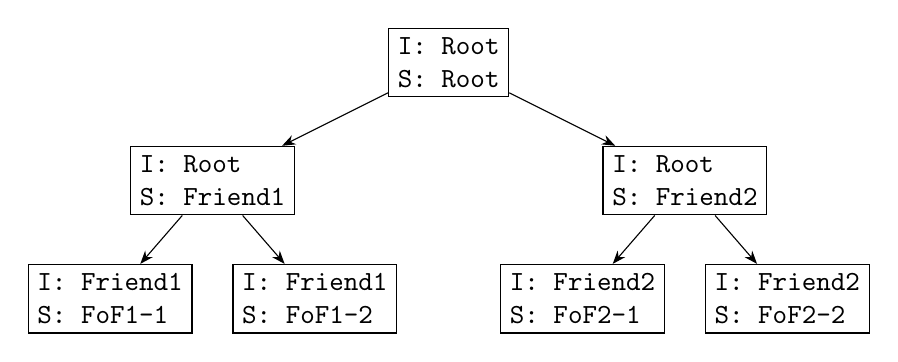
\begin{tikzpicture}
	\node (Root) at (0, 0) [align=left,draw] {\texttt{I: Root} \\ \texttt{S: Root}};
	\node (Friend1) at ($(Root) + (-3, -1.5)$) [align=left,draw] {\texttt{I: Root} \\ \texttt{S: Friend1}};
	\node (Friend2) at ($(Root) + (3, -1.5)$) [align=left,draw] {\texttt{I: Root} \\ \texttt{S: Friend2}};
	\node (FoF1-1) at ($(Friend1) + (-1.3, -1.5)$) [align=left,draw] {\texttt{I: Friend1} \\ \texttt{S: FoF1-1}};
	\node (FoF1-2) at ($(Friend1) + (1.3, -1.5)$) [align=left,draw] {\texttt{I: Friend1} \\ \texttt{S: FoF1-2}};
	\node (FoF2-1) at ($(Friend2) + (-1.3, -1.5)$) [align=left,draw] {\texttt{I: Friend2} \\ \texttt{S: FoF2-1}};
	\node (FoF2-2) at ($(Friend2) + (1.3, -1.5)$) [align=left,draw] {\texttt{I: Friend2} \\ \texttt{S: FoF2-2}};
	\draw[-Stealth] (Root) -- (Friend1);
	\draw[-Stealth] (Root) -- (Friend2);
	\draw[-Stealth] (Friend1) -- (FoF1-1);
	\draw[-Stealth] (Friend1) -- (FoF1-2);
	\draw[-Stealth] (Friend2) -- (FoF2-1);
	\draw[-Stealth] (Friend2) -- (FoF2-2);
\end{tikzpicture}
\end{center}

There are numerous problem with this architecture which the newer AFR PKI attempts to address.  First, the same certificates are used for both signing and authentication; this allows the potential vulnerability described in Schneier's book, ``Applied Cryptography'', section ``Resending the Message as a Receipt''.  While an amateur look at the TLS 1.3 protocol suggests that this attack isn't actually feasible, it seemed reasonable to mitigate the attack anyways due to the nature of public-private key cryptography.  Second, there were no extensions on any of the certificates issued by the root CA which would prevent a user from spoofing as the service (a rookie mistake).  Lastly, the root certificate's private key would have to exist on the running system in order for the service to authenticate itself to clients, meaning that a compromise of the service would result in the compromise of the entire PKI; while this situation isn't much improved with the AFR PKI due to the difficulty of re-issuing client certificates and revoking service certificates, a means of recovery could potentially be implemented in the future.  There are likely other flaws in this PKI which the author is not aware of.

\section{Future Work}

The current version and tooling around AFR is more of a proof-of-concept than anything that could be practically used in a large number of deployments.  Below are areas for potential research and improvements.

\subsection{Indirect CRLs}

First and foremost regarding features will need to be a working implementation of Indirect CRLs in order to implement Use Case \ref{admin-revoke-referred} (Admin revokes referrer certificate).  This appears to be a matter of setting the extensions \texttt{cRLDistributionPoints} and \texttt{DistributionPoint} in the end-entity (client) certificate and also setting the \texttt{IssuingDistributionPoint} extension's \texttt{indirectCRL} boolean to \texttt{TRUE} and creating corresponding \texttt{CertificateIssuer} entries in the signing CA's CRL.  There are a number of practical and protocol issues that prevented this from being implemented in the current tooling, though.

The first issue is that OpenSSL (1.1.1g) did not appear to support setting the \texttt{CertificateIssuer} extension in the CRLs generated via the \texttt{ca} command; this is likely in part because the CRL is generated from a plain text file database that does not have fields in which it can store information about certificates issued by other CAs.  While initial analysis suggests that the tools themselves support indirect CRLs, the mechanisms for generating one in the needed fashion do not appear to be a part of the command-line tools.  A second potential issue is that supporting indirect CRLs is optional for an X.509 PKI; this will likely not be an issue since this feature is of primary importance to the service, which can ensure support is enabled, and not the clients.  A third potential issue will be making sure that CRLs from both the referrer and signing certificate are processed; this may involve abusing the \texttt{reason} fields.  Fourth, a potential issue is that the \texttt{cRLDistributionPoint} extension must be placed in the referred certificate rather than the referrer certificate; what would happen if a referrer, through neglect or malevolence, left off this extension?  Finally, on the theoretical side, if using an actual network protocol for AFR (see below), it may make more sense to have the signing certificate issue all revocations; since the referrer needs to upload their CRL to the server anyways, the referrer could instead authenticate using the network protocol and then tell the signing certificate to revoke the specified referred certificate.

Getting Indirect CRLs working properly, or, more accurately, finding a way to implement Use Case \ref{admin-revoke-referred} is the biggest risk in getting this protocol to version 1.

\subsection{Network Protocol}

Contrary to all expectations, users are not thrilled when told that, in order to use AFR, they must type in a large number of arcane OpenSSL commands.  The current tooling around AFR is not particularly usable, so some way to make the PKI easier to use must be created if it is ever to be useful for a wider audience.  Perhaps the best way to implement this would be some kind of network protocol which could then be implemented by the end-user application.  The protocol may exist on a port separate from its corresponding service, or it may co-exist with the service (perhaps similar to how STARTTLS can co-exist with an existing protocol).  Certificate Signing Requests and Signed Certificates can be stored on a server as part of the protocol implementation in order to facilitate a central distribution location.  There's much that can be done here, but the rest will be left to speculation for now.

\subsection{Web Browser Plugin}

If a network protocol is created then it might make sense to have a web browser plugin which implements the protocol.  The plugin API would need to expose endpoints for overriding the default PKI of the browser on a per-site basis, though, otherwise foreign services from the default root CAs could Man-in-the-Middle the service connection, or the service could Man-in-the-Middle other sites which the user visits.  More research into the API of Web Extensions will be needed.

\subsection{Revoking Service Certificates}
\label{future-revoke-service}
There is currently no good way to revoke a service certificate such that the user properly rejects revoked service certificates.  Judging by the fact that most client applications do not appear to support protocols such as Online Certificate Status Protocol (OCSP), this does not appear to be a problem particular to the AFR PKI.

\subsection{Revoking Signing Certificates}

In case of disaster (a cracked service), some effort ought to be put into tooling that helps in the reissuing of certificates in the event of a signing certificate compromise.  Providing the admin a selection mechanism for certificates to reissue, perhaps based on the client's private key, and means to automatically store and reissue client and referrer certificates for successfully authenticated clients would seem to be a good path forward here, and could be implemented as part of the network protocol and service.

\subsection{PAM Integration}

It may make sense to write AFR as a Pluggable Authentication Module (PAM) so it can be plugged into a wide variety of services.  Or not.  More study of PAM is required here.

\subsection{Multiple Service Certificates}

The tooling should be developed further in order to provide support for multiple services.  It makes sense that one would have a single set of clients which are authorized for a plurality of services (such as IRC, Mumble, and mail, for example).  Each service should be provided a separate certificate so that the compromise of one service does not affect the other services.

\subsection{Link Friend and Referrer Certificates}

The link between friend and referrer certificates is currently implemented rather artificially in the tooling by file name conventions.  This will break down completely when certificates are re-issued, and it further has the problem that the metadata is not stored in the certificate itself.  There needs to be some mechanism to specify that a certificate belongs to a specific \emph{account}.  An optional extension to be added to the certificate would likely suffice here.  In addition, tools which are AFR-aware could then automatically map a client certificate to a specific account and log the user in appropriately, though this will be complicated by the fact that referrers may accidentally (or malevolently) issue accounts with the same names at the same time as other referrers, hence any account for a referred will need to be an amalgamation of the referrer account and the referred account.

\end{document}
